\subsection{Audio} \label{sec:audio}
Für die Audioausgabe sind auch Hardware Komponenten notwendig. In diesem Kapitel werden alle einzelnen Komponenten welche für die Audioausgabe notwendig sind genauer erläutert. Es umfasst zum einen die Aufbereitung des Audio Signals (Unterkapitel LC-Filter), ebenso umfasst es die Verstärkung des Signals (Unterkapitel Verstärkerstufe) und zu guter Schluss die Komponente welche für die Audioausgabe zuständig ist (Abschnitt Knochenschallaktor).

\subsubsection*{LC-Filter}\label{sec:schutzeinrichtung}
Vor dem Audioverstärker wird noch ein Filter benötigt, welcher das PWM Signal des Microcontrollers filtert und den DC Anteil entfernt. Um den Microcontroller zu entkoppeln ist ein $100\mu F$ Elektrolytkondensator an jedem PWM Ausgang in Serie geschalten. Das Filter wurde wie folgt dimensioniert. 
\begin{equation}
f_g = \frac{1}{2\cdot \pi \cdot \sqrt{L\cdot C}}
\label{eq LC Filter}
\end{equation}

Um die Gleichung zu lösen wurde eine Grenzfrequenz ($f_g$) von $20kHz$ angenommen und ein Kondensator (C) von $1\mu F$ gewählt. Daraus ergibt sich die Gleichung \ref{eq LC Filter nach L}. 
\begin{equation}
L = \frac{1}{(2\cdot \pi \cdot f_g)^2\cdot C } = 63.33\mu H
\label{eq LC Filter nach L}
\end{equation}
Daraus wurde dann eine L mit dem Wert $68\mu H$ gewählt. Setzt man die Werte in Gleichung \ref{eq LC Filter} ein ergibt sich eine Grenzfrequenz von $19.3kHz$. 


\subsubsection*{Verstärkerstufe} \label{sec:verstaerkerstufe}
Nachdem die Steuerungseinheit gezeigt wurde, kann nun die Ausgangsstufe erläutert werden. Mit einer Verstärkerstufe lassen sich auf einfache Art und Weise Signale jeglicher Form verstärken. Sie eignen sich bestens, um den Ausgang eines Mikrocontrollers entsprechend aufzubereiten, da die Ausgangsseite meist sehr niedrige Ströme aufweist. Dadurch kann dem Knochenschallaktor genügend Energie zur Verfügung gestellt werden. Prinzipiell gibt es zwei Arten von Verstärkern. Entweder erfolgt die Umsetzung digital oder analog. Beide erfüllen die gleiche Aufgabe, weisen jedoch bezüglich Wirkungsgrad einen deutlichen Unterschied auf. Die digitale Variante weist ungefähr einen Wirkungsgrad von 90$\%$ auf \cite{BoneConductorAdafruit}, während die analoge Variante einen maximalen Wirkungsgrad im Bereich der Leistungsanpassung erzielt \cite{Niklaus_Skript}. Aus diesem Grund wird ein digitaler Verstärker (Class-D-Verstärker) in der Anwendung implementiert. Die Wahl fiel auf den Stereo-Amplifier MAX 98306. Der Verstärker hat einen Stromverbrauch von $143mA$ und eine Speisespannung von $3.3V$. Somit hat er einen Leistungsverbrauch von $471.9 mW$. Im Standby benötigt er lediglich $2 mA$ und somit $6.6 mW$\cite{Verstaerker}.


\subsubsection*{Knochenschallaktor} \label{sec:knochenschallaktor}
Nachdem das vom Mikrocontroller ausgegebene Audio-File über die Verstärkerstufe entsprechend aufbereitet wurde, kann nun die Audiodatei über einen sogenannten Knochenschallaktor ausgegeben werden.
Der Aktor arbeitet nach dem Prinzip der Weiterleitung von Schall-Schwingungen oder auch Vibrationen. Dadurch lässt sich der ursprüngliche Gehörgang umgehen und die Schwingungen werden über den Schädelknochen an das Innenohr übertragen. Dies verbessert auch die Hygiene der Anwendung, da kein direkter Kontakt mit dem Gehörgang stattfindet.\cite{Knochenschall}
Für die Anwendung im Dōjō wird ein Knochenschallaktor des Herstellers Adafruit verwendet, welcher in der Abbildung \ref{fig:knochenschallAda} ersichtlich ist.

\begin{figure}[H]
	\begin{center}
		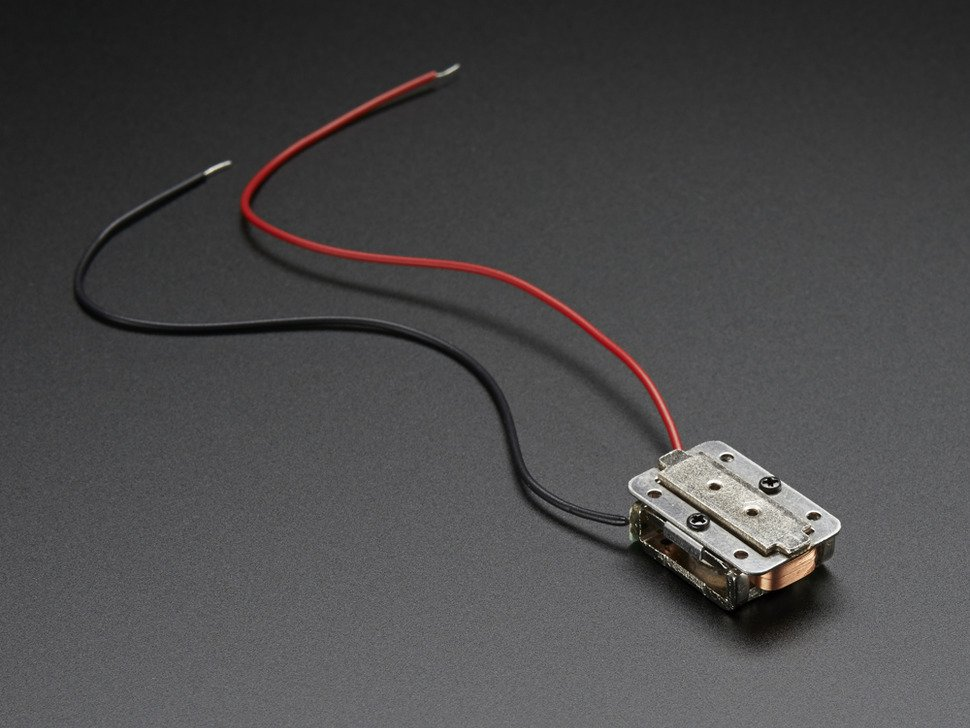
\includegraphics[width=120mm]{data/KnochenschallaktorAdafruit1.jpg}
		\caption[Knochenschallaktor \cite{BoneConductorAdafruit}]{Knochenschallaktor von Adafruit} %picture caption
		\label{fig:knochenschallAda}
	\end{center}
\end{figure}

Das ausgewählte Bauteil eignet sich bestens für die Verwendung im Dōjō. Mit einem Gewicht von 9.6 g und den Dimensionen 14x21,5x7,9 lässt sich der Aktor gut in das bestehende Gehäuse implementieren \cite{BoneConductorAdafruit}. Weiter ist das Bauteil relativ kostengünstig im Handel erhältlich und kann $1W_{RMS}$ Leistung liefern, was sich dann in der Lautstärke bemerkbar macht. Nach ausführlichen Recherchearbeiten konnten keine wirklichen Alternativen ausgemacht werden. Meist befindet sich die Technologie noch in der Entwicklungsphase oder fällt aufgrund des Preises aus der Auswahlmöglichkeit.
